% \clearpage
\section{Results}

% \Cref{fig:benchmark_bars} shows HRM's performance on the Sudoku, Maze, ARC-AGI-1 and ARC-AGI-2 tasks. 
This section begins by describing the ARC-AGI, Sudoku, and Maze benchmarks, followed by an overview of the baseline models and their results. \Cref{fig:benchmark_intro}-(a,b,c) presents a visual representation of the three benchmark tasks, which are selected to evaluate various reasoning abilities in AI models.

\subsection{Benchmarks}

\begin{figure}[t]
    \centering
    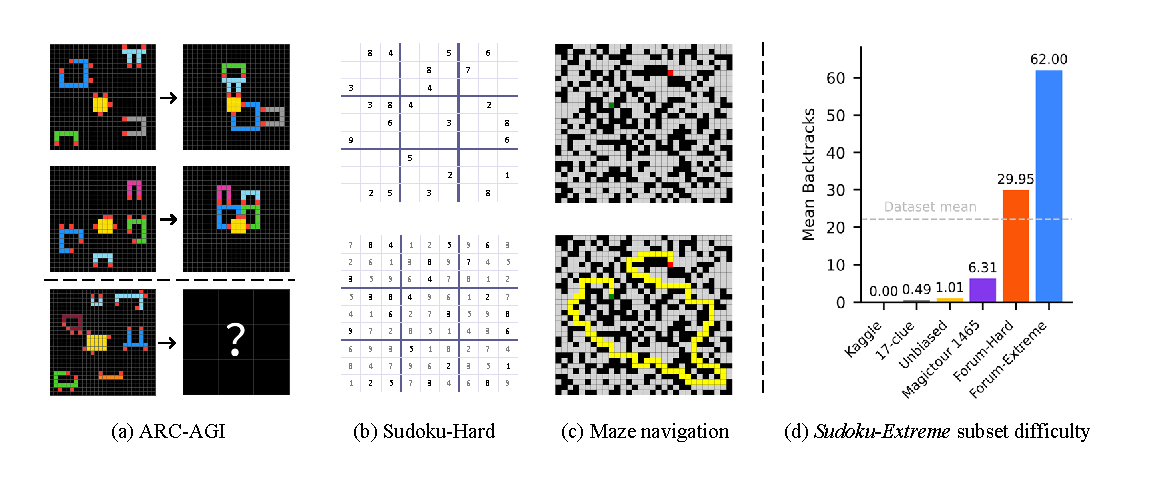
\includegraphics[width=1\linewidth]{figures/benchmark_bars/dataset_intro.pdf}
    \caption{\textbf{Left:} Visualization of benchmark tasks. \textbf{Right:} Difficulty of \textit{Sudoku-Extreme} examples.}
    \label{fig:benchmark_intro}
\end{figure}

%\todoy{In \Cref{fig:benchmark_intro}-(d): \textit{Sudoku-Extreme} --> \textit{Sudoku-Extreme-Full}? }\cmtone{There are two sizes - "Full" refers to 3.8M for analysis experiments to prevent overfitting, while the set for main experiments are 1000 samples}

\textbf{ARC-AGI Challenge}~ The ARC-AGI benchmark evaluates general fluid intelligence through IQ-test-like puzzles that require inductive reasoning~\cite{AbstractionReasoning2019}. The initial version, ARC-AGI-1, presents challenges as input-output grid pairs that force AI systems to extract and generalize abstract rules from just a few examples. Each task provides a few input–output example pairs (usually 2–3) and a test input. An AI model has two attempts to produce the correct output grid. Although some believe that mastering ARC-AGI would signal true artificial general intelligence, its primary purpose is to expose the current roadblocks in AGI progress. In fact, both conventional deep learning methods and CoT techniques have faced significant challenges with ARC-AGI-1, primarily because it requires the ability to generalize to entirely new tasks~\citep{Chollet2024ARCP2}.

Addressing the limitations identified in ARC-AGI-1, ARC-AGI-2 significantly expands the benchmark by providing a more comprehensive and carefully refined collection of tasks. These new tasks emphasize deeper compositional reasoning, multi-step logic, contextual rule application, and symbolic abstraction. Human calibration studies show these tasks are challenging but doable for people, while being much harder for current AI systems, offering a clearer measure of general reasoning abilities~\citep{Chollet2025ARCAGI2AN}.

\textbf{Sudoku-Extreme}~ Sudoku is a 9$\times$9 logic puzzle, requiring each row, column, and 3$\times$3 block to contain the digits 1–9 exactly once. A prediction is considered correct if it exactly matches the puzzle's unique solution. Sudoku's complex logical structure makes it a popular benchmark for evaluating logical reasoning in machine learning~\citep{Palm2017RecurrentRN,Long2023LargeLM,Du2024LearningIR}.

The most frequently used Sudoku dataset in research, namely the Kaggle dataset~\citep{sudoku2018}, can be fully solved using elementary single-digit techniques~\citep{SDT-Sudoku}. The minimal 17-clue puzzles~\citep{Palm2017RecurrentRN}, another widely-used collection, might seem more challenging due to its small number of clues. However, this perception is misleading---since 17 represents the minimum number of clues required to guarantee a unique Sudoku solution, these hints need to be highly orthogonal to each other. This orthogonal arrangement leads to many direct, easily-resolved solution paths~\cite{tdoku}.

We introduce \textit{Sudoku-Extreme}, a more challenging dataset that is compiled from the aforementioned easy datasets as well as puzzles recognized by the Sudoku community as exceptionally difficult for human players:
\begin{itemize}
    \item Easy puzzles compiled from Kaggle, 17-clue, plus unbiased samples from the Sudoku puzzle distribution~\cite{tdoku}: totaling \num{1149158} puzzles.
    \item Challenging puzzles compiled from Magictour 1465, Forum-Hard and Forum-Extreme subsets: totaling \num{3104157} puzzles.
\end{itemize}
The compiled data then undergo a strict 90/10 train-test split, ensuring that the test set puzzles cannot be derived through equivalent transformations of any training samples. \textit{Sudoku-Extreme} is a down-sampled subset of this data containing 1000 training examples. We use \textit{Sudoku-Extreme}  in our main experiments (\Cref{fig:benchmark_bars}), which focuses on small-sample learning scenarios. To guarantee convergence and control overfitting effects in our analysis experiments (\Cref{fig:perf-layers,fig:forward-residual,fig:act}), we use the complete training data, \textit{Sudoku-Extreme-Full}, containing \num{3831994} examples.

%For the analysis experiments presented in \Cref{fig:perf-layers,fig:forward-residual,fig:act}, we trained all models on the complete training data, \textit{Sudoku-Extreme-Full}, containing \num{3831994} examples. This approach was taken to ensure convergence and to control for the influence of overfitting that can be present in smaller sample sizes, thereby highlighting the effect of effective depth.


We measure puzzle difficulty by counting the number of search backtracks (``guesses'') required by a smart Sudoku solver program \textit{tdoku}, which uses propositional logic to reduce the number of guesses~\citep{tdoku}. Our \textit{Sudoku-Extreme} dataset exhibits a mean difficulty of $22$ backtracks per puzzle, significantly higher than existing datasets, including recent handmade puzzles Sudoku-Bench \citep{Seely2025SudokuBenchEC} which average just $0.45$ backtracks per puzzle. These subset complexity levels are shown in~\Cref{fig:benchmark_intro}-(d).
%\cmtone{tdoku is highly optimized with symbolic heuristic-search, so little backtracks are needed, compared to millions in brute-force DFS. Should we mention that?}

\textbf{Maze-Hard} This task involves finding the optimal path in a 30$\times$30 maze, making it interpretable and frequently used for training LLMs in search tasks \citep{Darlow2025ContinuousTM, dualformer2025, searchformer2024}. %It is typically solved using tree-search algorithms such as A*.
We adopt the instance generation procedure of \citet{searchformer2024}, but introduce an additional filter to retain only those instances whose difficulty exceeds 110. Here, ``difficulty'' is defined as the length of the shortest path, which aligns with the linear time complexity of the wavefront breadth-first search algorithm on GPUs~\citep{wavefrontBFS}. A path is considered correct if it is valid and optimal---that is, the shortest route from the start to the goal. The training and test set both include 1000 examples.

\subsection{Evaluation Details}

For all benchmarks, HRM models were initialized with random weights and trained in the sequence-to-sequence setup using the input-output pairs. The two-dimensional input and output grids were flattened and then padded to the maximum sequence length. The resulting performance is shown in \Cref{fig:benchmark_bars}. Remarkably, HRM attains these results with just \textasciitilde1000 training examples per task---and \textbf{without pretraining or CoT labels}.

For ARC-AGI challenge, we start with all input-output example pairs in the training and the evaluation sets. The dataset is augmented by applying translations, rotations, flips, and color permutations to the puzzles. Each task example is prepended with a learnable special token that represents the puzzle it belongs to. At test time, we proceed as follows for each test input in the evaluation set: (1) Generate and solve 1000 augmented variants and, for each, apply the inverse‐augmentation transform to obtain a prediction. (2) Choose the two most popular predictions as the final outputs.\footnote{The ARC-AGI allows two attempts for each test input.} All results are reported on the evaluation set.

%At test time, we first augment each test example 1000 times and obtain the corresponding predictions by an inverse augmentation transform, and then obtain the majority vote for the two trials allowed for each test sample~\citep{Chollet2025ARCAGI2AN}. Performance is reported on the evaluation set.

We augment Sudoku puzzles by applying band and digit permutations, while data augmentation is disabled for Maze tasks. Both tasks undergo only a single inference pass.

For ARC-AGI, the scores of the CoT models are taken from the official leaderboard~\citep{Chollet2025ARCAGI2AN}, while for Sudoku and Maze, the scores are obtained by evaluating through the corresponding API.

%The scores of the CoT models are taken from the official leaderboard for ARC-AGI \citep{Chollet2025ARCAGI2AN}, and evaluated using API for Sudoku and Maze.

In \Cref{fig:benchmark_bars}, the baselines are grouped based on whether they are pre-trained and use CoT, or neither. The ``Direct pred'' baseline means using ``direct prediction without CoT and pre-training'', which retains the exact training setup of HRM but swaps in a Transformer architecture. Interestingly, on ARC-AGI-1, ``Direct pred'' matches the performance of \citet{liao2025arcagiwithoutpretraining}, who built a carefully designed, domain-specific equivariant network for learning the ARC-AGI task from scratch, without pre-training. By substituting the Transformer architecture with HRM's hierarchical framework and implementing ACT, we achieve more than a twofold performance improvement.

On the \textit{Sudoku-Extreme} and \textit{Maze-Hard} benchmarks, the performance gap between HRM and the baseline methods is significant, as the baselines almost never manage to solve the tasks. These benchmarks that demand lengthy reasoning traces are particularly difficult for CoT-based methods. With only 1000 training examples, the ``Direct pred'' baseline---which employs an 8-layer Transformer identical in size to HRM---fails entirely on these challenging reasoning problems. When trained on the larger \textit{Sudoku-Extreme-Full} dataset, however, ``Direct pred'' can solve some easy Sudoku puzzles and reaches $16.9\%$ accuracy (see \Cref{fig:perf-layers}). \citet{searchformer2024} showed that a large vanilla Transformer model with 175M parameters, trained on 1 million examples across multiple trials, achieved only marginal success on 30x30 Maze tasks, with accuracy below $20\%$ using the $pass@64$ evaluation metric.


% \todoy[inline]{Say something about "Direct pred" and why it performs so poorly. I assume it is DEQ using a transformer with 8 layers, which is very similar to HRM configuration with H=2/8 and L=1 (see Heatmap figure "Planner only"). One difference between "Direct pred" and "Planner only" is that in HRM, z_H update includes its previous value too. Does this explain their performance gap? }

\subsection{Visualization of intermediate timesteps}

\begin{figure}[t]
\centering
\includegraphics[width=\linewidth]{figures/forward_res/trajectory_plot.pdf}
\caption{Comparison of forward residuals and PCA trajectories. HRM shows hierarchical convergence: the H-module steadily converges, while the L-module repeatedly converges within cycles before being reset by H, resulting in residual spikes. The recurrent neural network exhibits rapid convergence with residuals quickly approaching zero. In contrast, the deep neural network experiences vanishing gradients, with significant residuals primarily in the initial (input) and final layers.}
\label{fig:forward-residual}
\end{figure}


% <decode intermediate results: at each timestep $i$, using a premature forward of H, $f_O(f_H(z_H^i, z_L^i; \theta_H); \theta_O)$ to decode>

% <diverse solutions modes>

% Sudoku: search-like trial-and-error process. Then refine.

% Maze: exploring multiple candidate paths in parallel, prune blocked or suboptimal paths, followed by several refining rounds.

% ARC: solve the puzzle gradually and refining.

Although HRM demonstrates strong performance on complex reasoning tasks, it raises an intriguing question: what underlying reasoning algorithms does the HRM neural network actually implement? Addressing this question is important for enhancing model interpretability and developing a deeper understanding of the HRM solution space. 

While a definitive answer lies beyond our current scope, we begin our investigation by analyzing state trajectories and their corresponding solution evolution. More specifically, at each timestep $i$ and given the low-level and high-level state pair ($z_L^i$ and $z_H^i$) we perform a preliminary forward pass through the H-module to obtain $\bar{z}^{i} = f_H(z_H^i, z_L^i; \theta_H)$ and its corresponding decoded prediction $\bar{y}^{i} = f_O(\bar{z}^{i}; \theta_O)$. The prediction $\bar{y}^{i}$ is then visualized in \Cref{fig:visualization}.   

% First, HRM seems to employ a diverse set of strategies in solving different reasoning problems.
In the Maze task, HRM appears to initially explore several potential paths simultaneously, subsequently eliminating blocked or inefficient routes, then constructing a preliminary solution outline followed by multiple refinement iterations. In Sudoku, the strategy resembles a depth-first search approach, where the model appears to explore potential solutions and backtracks when it hits dead ends. HRM uses a different approach for ARC tasks, making incremental adjustments to the board and iteratively improving it until reaching a solution. Unlike Sudoku, which involves frequent backtracking, the ARC solution path follows a more consistent progression similar to hill-climbing optimization. 
 
Importantly, the model shows that it can adapt to different reasoning approaches, likely choosing an effective strategy for each particular task. Further research is needed to gain more comprehensive insights into these solution strategies.
